\chapter{Evaluación del Método mediante Resampleo en \emph{Trackfiles}}
\label{chap:evaluacion-trackfiles}

\section{Metodología del análisis}
\label{sec:metodologia-analisis}

Para validar el método propuesto, se remuestrearon \emph{trackfiles} generados en simulaciones Monte Carlo previas y se compararon los \emph{trackfiles} obtenidos contra los originales. Estos archivos constituyen conjuntos de datos representativos que permiten verificar si la metodología implementada es capaz de aproximar adecuadamente las distribuciones y correlaciones originales del espacio de fases ($\mathbf{E}$–$\mathbf{r}$–$\boldsymbol{\Omega}$).

La estrategia general consiste en aplicar el método a tres \emph{trackfiles} diferentes, utilizando distintos esquemas de configuración. En cada caso se varían parámetros como el orden de las variables, el número de macrogrupos y microgrupos, y se analiza su impacto en la calidad de la reconstrucción. Además, se contempla la posibilidad de definir manualmente los bordes de los macrogrupos en aquellas variables donde la información previa sobre la geometría o el comportamiento de las partículas permita mejorar la separación de poblaciones con características distintas.

Los principales aspectos del análisis son los siguientes:

\begin{itemize}
    \item \textbf{Orden de variables:} se considera cómo el orden en que se procesan las variables afecta a la fragmentación del \emph{trackfile} original en subconjuntos y, por ende, a la estadística de cada variable de procesamiento, que disminuye a medida que aumentan los macrogrupos. En general, la primera variable se beneficia de la estadística total, debido a que todavía no se ha subdividido en sucesivos subconjuntos, mientras que las siguientes reciben subconjuntos progresivamente más pequeños. Dado que la variable $\phi$ suele presentar una distribución cercana a uniforme en sistemas con simetría, se ha elegido colocarla en la última posición.
    
    \item \textbf{Cantidad de macrogrupos:} se comparan esquemas uniformes (por ejemplo, $[8,8,8,8]$, $[6,6,6,6]$) y esquemas crecientes o decrecientes (como $[9,8,7,6]$, $[6,7,8,9]$). Esta elección impacta en la capacidad de representar correlaciones sin introducir exceso de ruido estadístico.
    
    \item \textbf{Cantidad de microgrupos:} se estudia el efecto de aumentar o disminuir la resolución dentro de cada macrogrupo.
\end{itemize}

Para el primer \emph{trackfile} analizado se analizan los diferentes estilos de bineado, que pueden ser de igual ancho, de igual integral o adaptativo, tanto para la definición de los bines de los macrogrupos y microgrupos. Los tres esquemas permiten obtener diferentes aproximaciones de la misma distribución original.

Para cada configuración de entrada se comparan visualmente las distribuciones 1D y 2D obtenidas, analizando las distribuciones y sus errores relativos, como así también se analiza la divergencia KL obtenida para los casos 1D y 2D.

\begin{itemize}
    \item \textbf{Distribuciones 1D}: se comparan las distribuciones de cada variable remuestreadas utilizando el método implementado contra las originales del \emph{trackfile}. 
    \item \textbf{Correlaciones 2D}: se representan visualmente mediante mapas de error relativo entre las matrices de correlación originales y las reconstruidas a través del remuestreo.
    \item \textbf{Métrica cuantitativa}: se utiliza la divergencia de Kullback-Leibler (KL) como estimador numérico de la diferencia entre las distribuciones, permitiendo comparar configuraciones de forma objetiva.
\end{itemize}
% En algun momento hay que explicar que el KL requiere que no haya valores 0 y requiere discretizar la muestra. Lo que se hizo fue sumarle 1e-9 a todos los bines antes de normalizar. Es tecnica de pseudoconteo. Ademas se han tomado 1000 bines para los casos 1D y 1000x1000 bines para los casos 2D. esto se ha dejado fijo porque al variar estos parametros valia la salida del KL. Por lo tanto para poder comparar entre distintos casos se ha dejado fijo.

\section{Análisis del Trackfile 1: haz colimado en tubo de vacío}

El primer trackfile analizado fue proporcionado externamente. Corresponde a partículas registradas en una superficie ubicada dentro de un tubo de vacío rodeado por agua. La lista contiene únicamente neutrones que atraviesan la sección del canal, lo cual se corrobora en la proyección $x$-$y$, donde se observa una distribución uniforme contenida en un cuadrado, correspondiente a la sección del tubo. La figura \ref{fig:trackfile1_x_y} muestra la proyección de los neutrones en el plano $x$-$y$.

\begin{figure}[h]
    \centering
    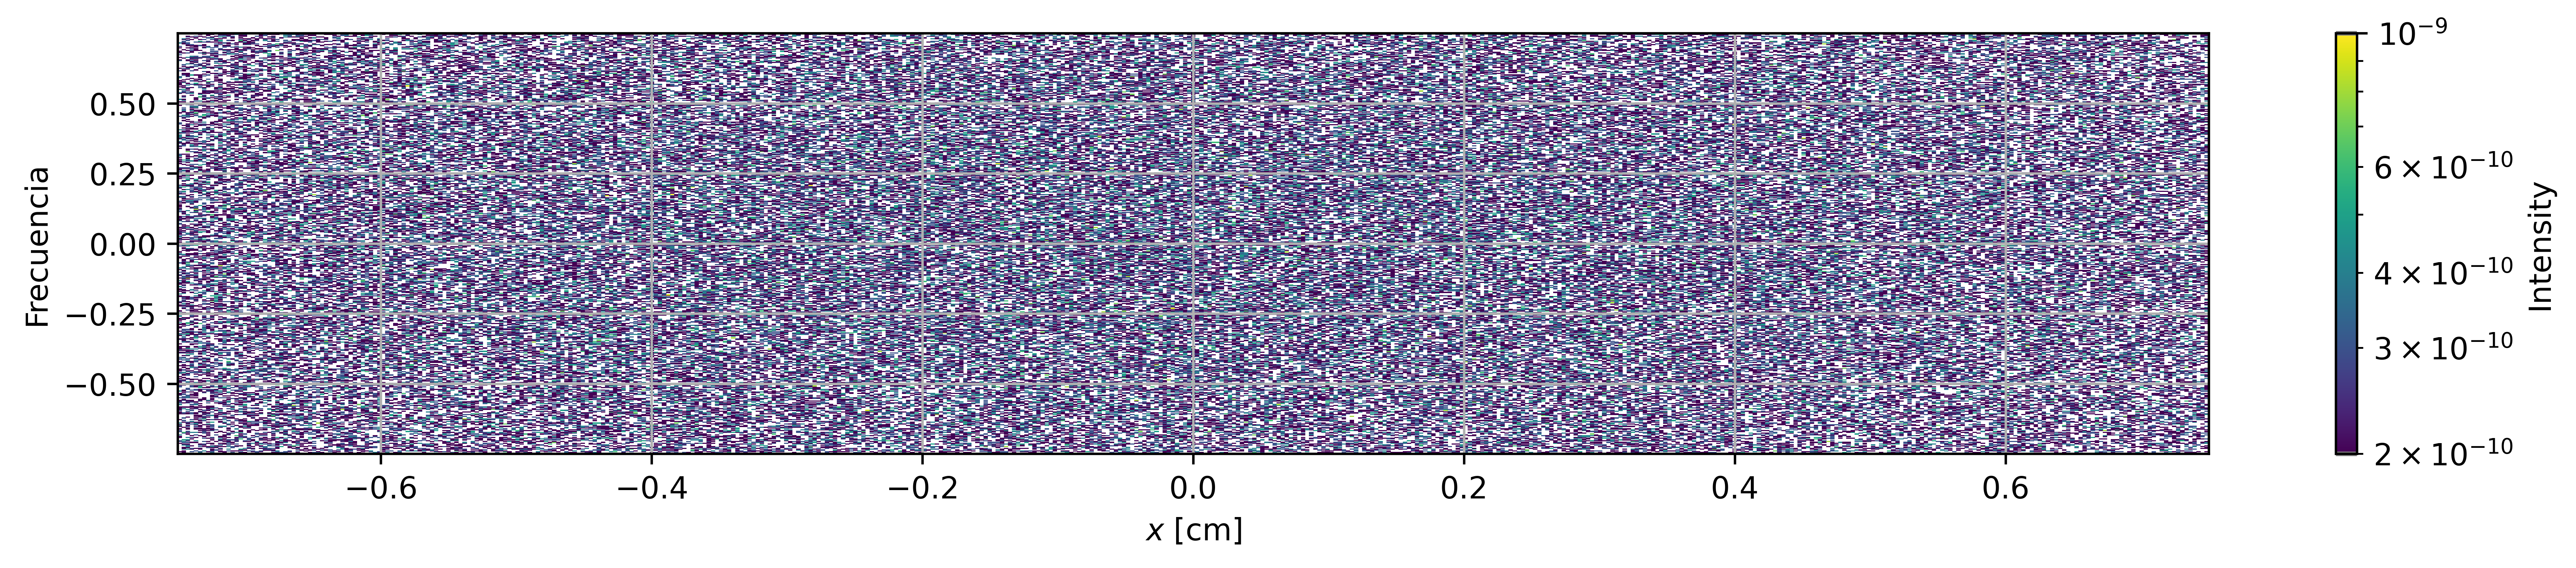
\includegraphics[width=\textwidth]{figs/fig2_2.png}
    \caption{Distribuciones de $x$ vs $y$ para el primer trackfile. Se observa uniformidad en toda la sección del tubo.}
    \label{fig:trackfile1_x_y}
\end{figure}

Este conjunto contiene dos poblaciones de neutrones claramente diferenciadas. La primera corresponde a neutrones que no han sufrido colisiones: todos ellos poseen dirección $\mu = 1$ y una letargia mínima fija, sin dispersión alguna, lo cual indica que la fuente original fue configurada con estos valores de forma determinista. La segunda población incluye neutrones que han colisionado: en este caso, las distribuciones de $\mu$ y letargia son más amplias y continuas, reflejando la dispersión introducida por las interacciones. Este comportamiento se observa en la figura \ref{fig:trackfile1_letargia_mu}, donde se presentan las distribuciones de letargia y $\mu$ para el primer trackfile. 

\begin{figure}[h]
    \centering
    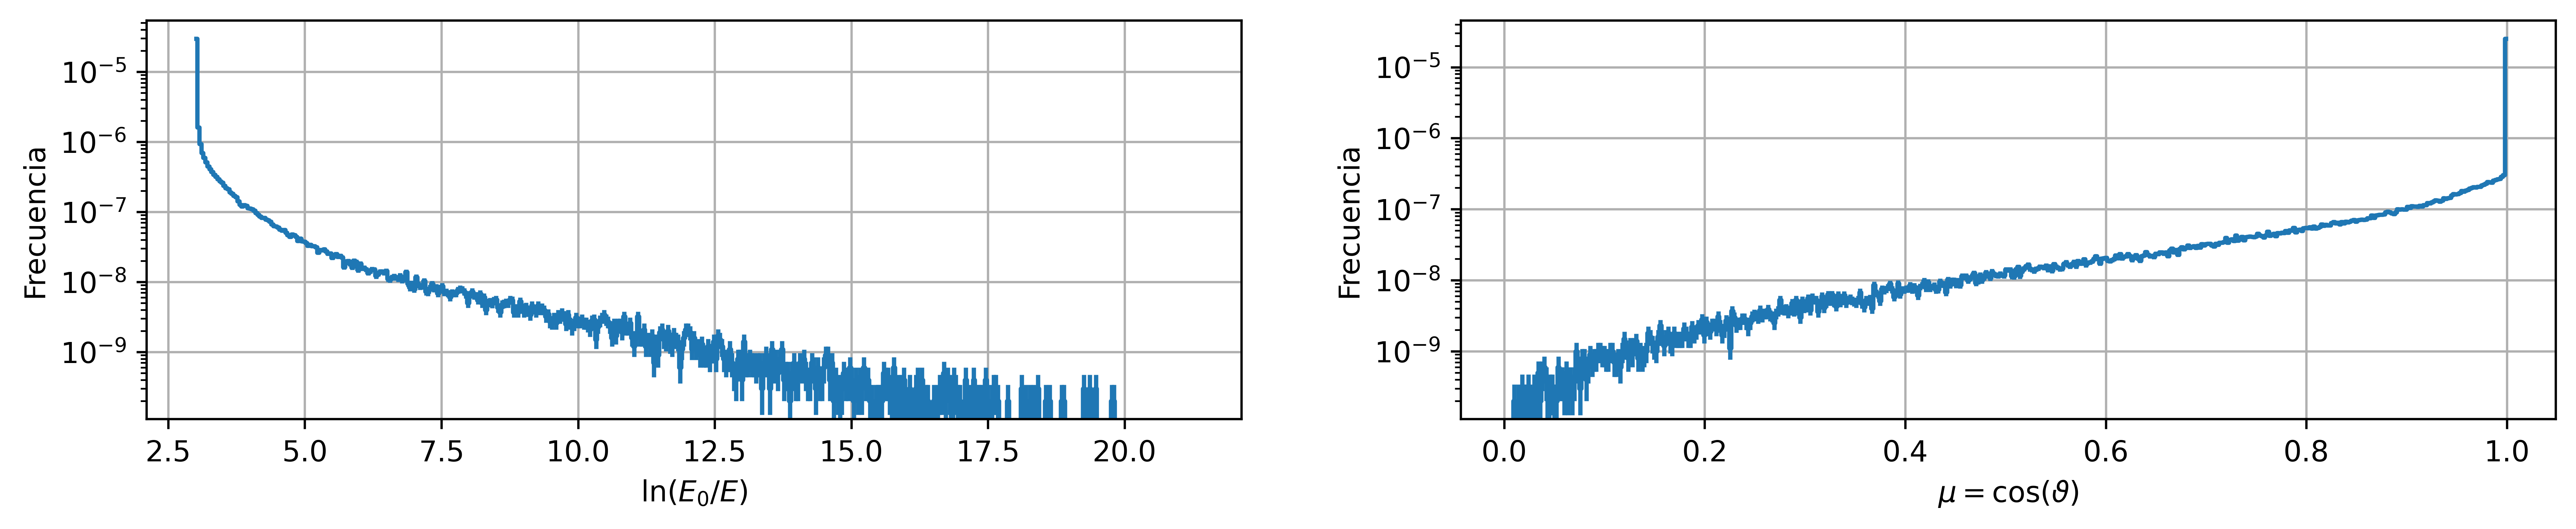
\includegraphics[width=\textwidth]{figs/fig2_1.png}
    \caption{Distribuciones de letargia y $\mu$ para el primer trackfile, con escala logaritmica en el eje y. Se observa la presencia de dos poblaciones: una concentrada en $\mu = 1$ y letargia mínima, montada sobre una distribución continua de neutrones colisionados.}
    \label{fig:trackfile1_letargia_mu}
\end{figure}

Esta doble estructura se evidencia particularmente en los gráficos 2D de letargia vs. $\mu$, donde ambas poblaciones forman conjuntos visualmente separados (de hecho estamos hablando de dos conjuntos distintos. Repensar esto). Ver figura \ref{fig:trackfile1_letargia_mu_2}. Este fenómeno plantea un desafío para los métodos de muestreo, al requerir una representación precisa tanto de distribuciones concentradas tipo delta como de distribuciones extendidas y sus correlaciones.

\begin{figure}[h]
    \centering
    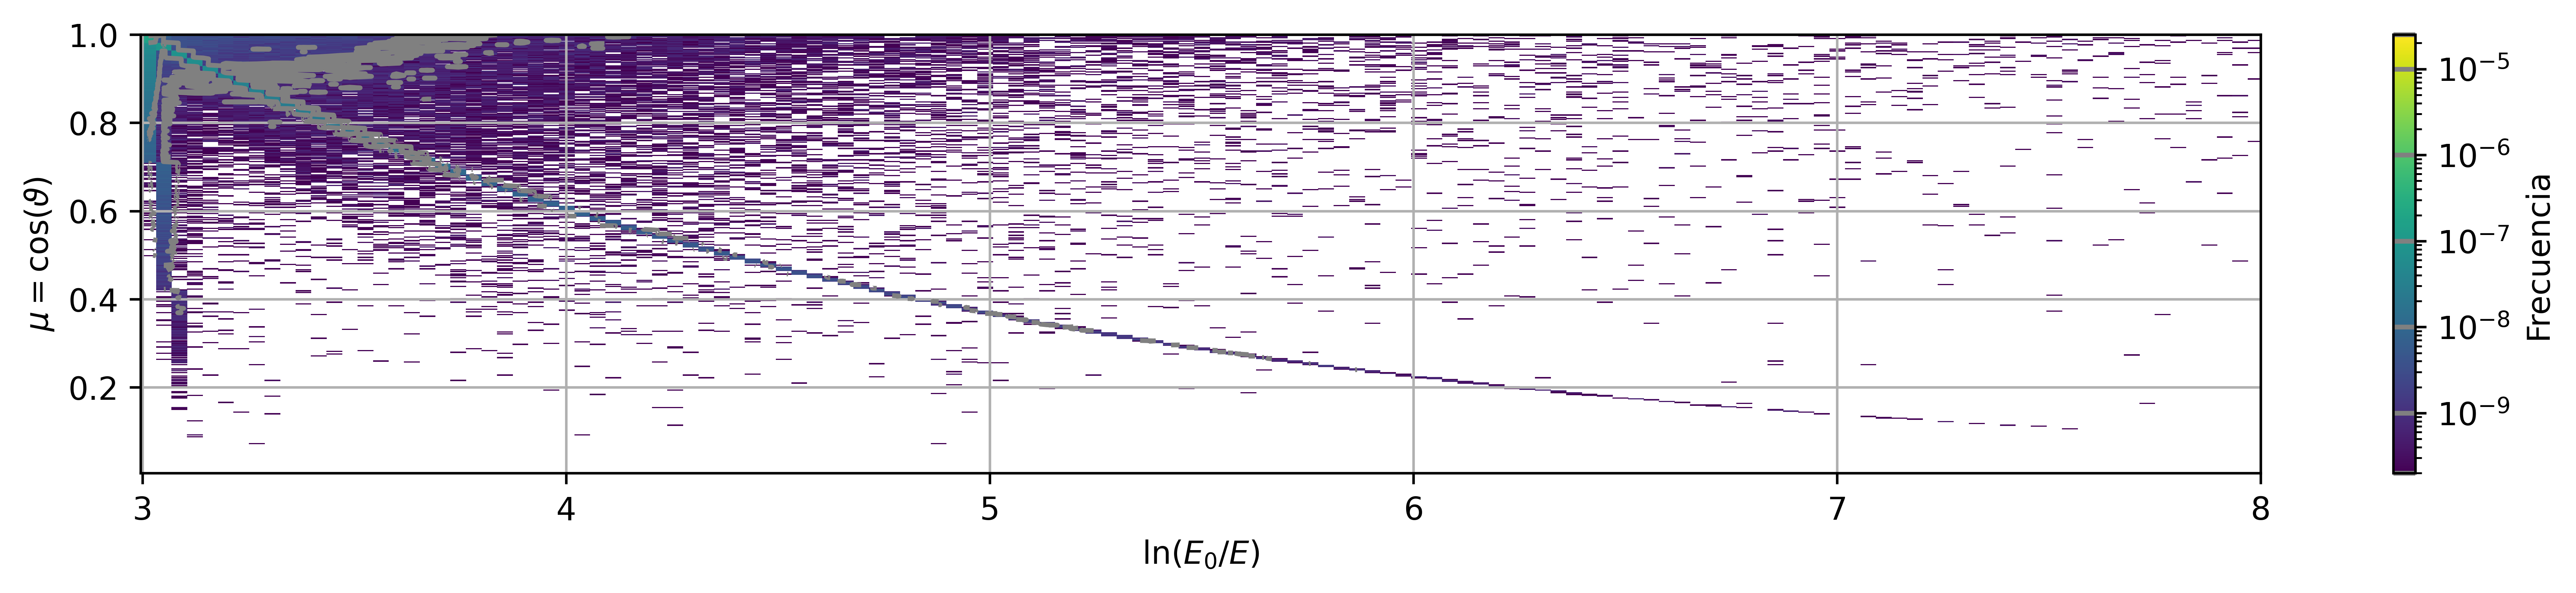
\includegraphics[width=\textwidth]{figs/fig2_3.png}
    \caption{Distribuciones de letargia vs $\mu$ para el primer trackfile. Se observa la presencia de un conjunto de neutrones graficados como una linea sobre una distribucion uniforme de fondo.}
    \label{fig:trackfile1_letargia_mu_2}
\end{figure}

\subsection{Configuración 1: bineado micro y macro uniforme}  
Se empleó una configuración con macrogrupos y microgrupos de ancho uniforme. Se seleccionaron $n_{\text{macro}} = 8$ y $n_{\text{micro}} = 100$ para cada variable, en el orden de variables: \texttt{[ln(E0/E), x, y, mu, phi]}. Esta configuración permite evaluar el desempeño base sin ningún tipo de adaptación.

Visualmente, se observa que la distribución tipo delta en letargia mínima y $\mu = 1$ es reemplazada por un rectángulo con el ancho del bin, perdiéndose el detalle de los picos originales. El efecto del resampleo mediante bins uniformes se puede ver en las figuras \ref{fig:trackfile1_config1_letargia} y \ref{fig:trackfile1_config1_mu}, donde se comparan las distribuciones de letargia y $\mu$ entre el trackfile original y el remuestreado.

\begin{figure}[h]
    \centering
    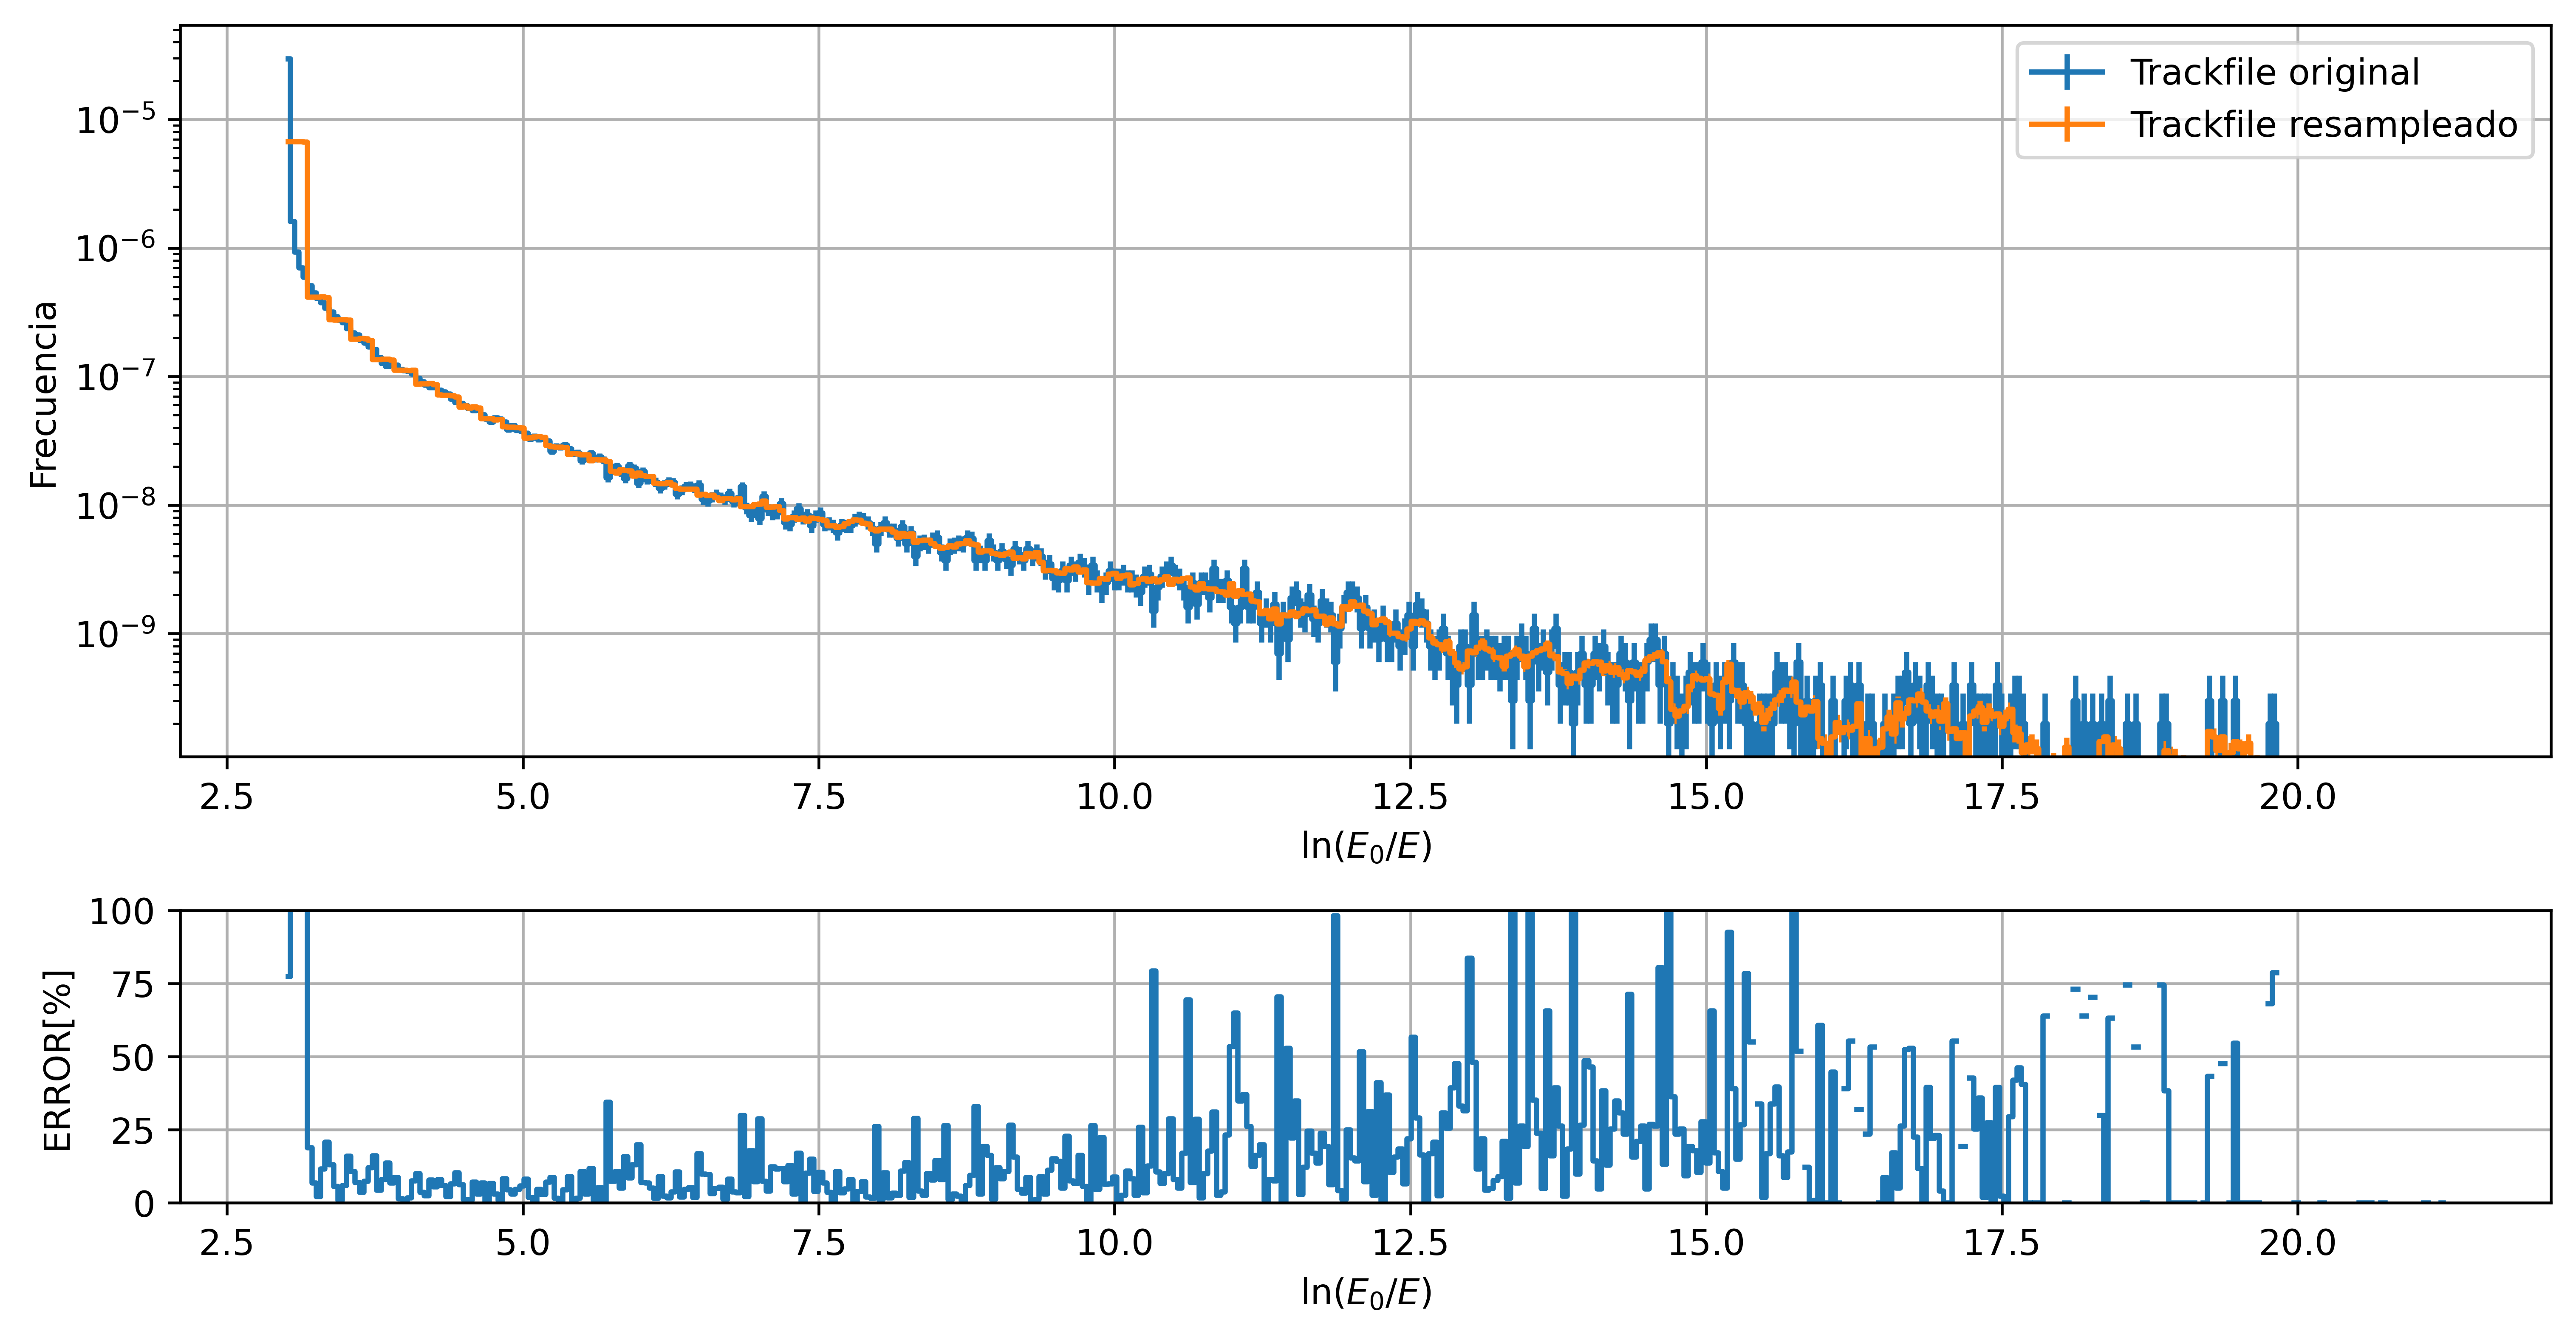
\includegraphics[width=\textwidth]{figs/fig2_4.png}
    \caption{Comparacion de la distribucion de letargia entre el trackfile original y el trackfile remuestreado. Se observa el efecto de la discretizacion uniforme en la distribucion de letargia.}
    \label{fig:trackfile1_config1_letargia}
\end{figure}

\begin{figure}[h]
    \centering
    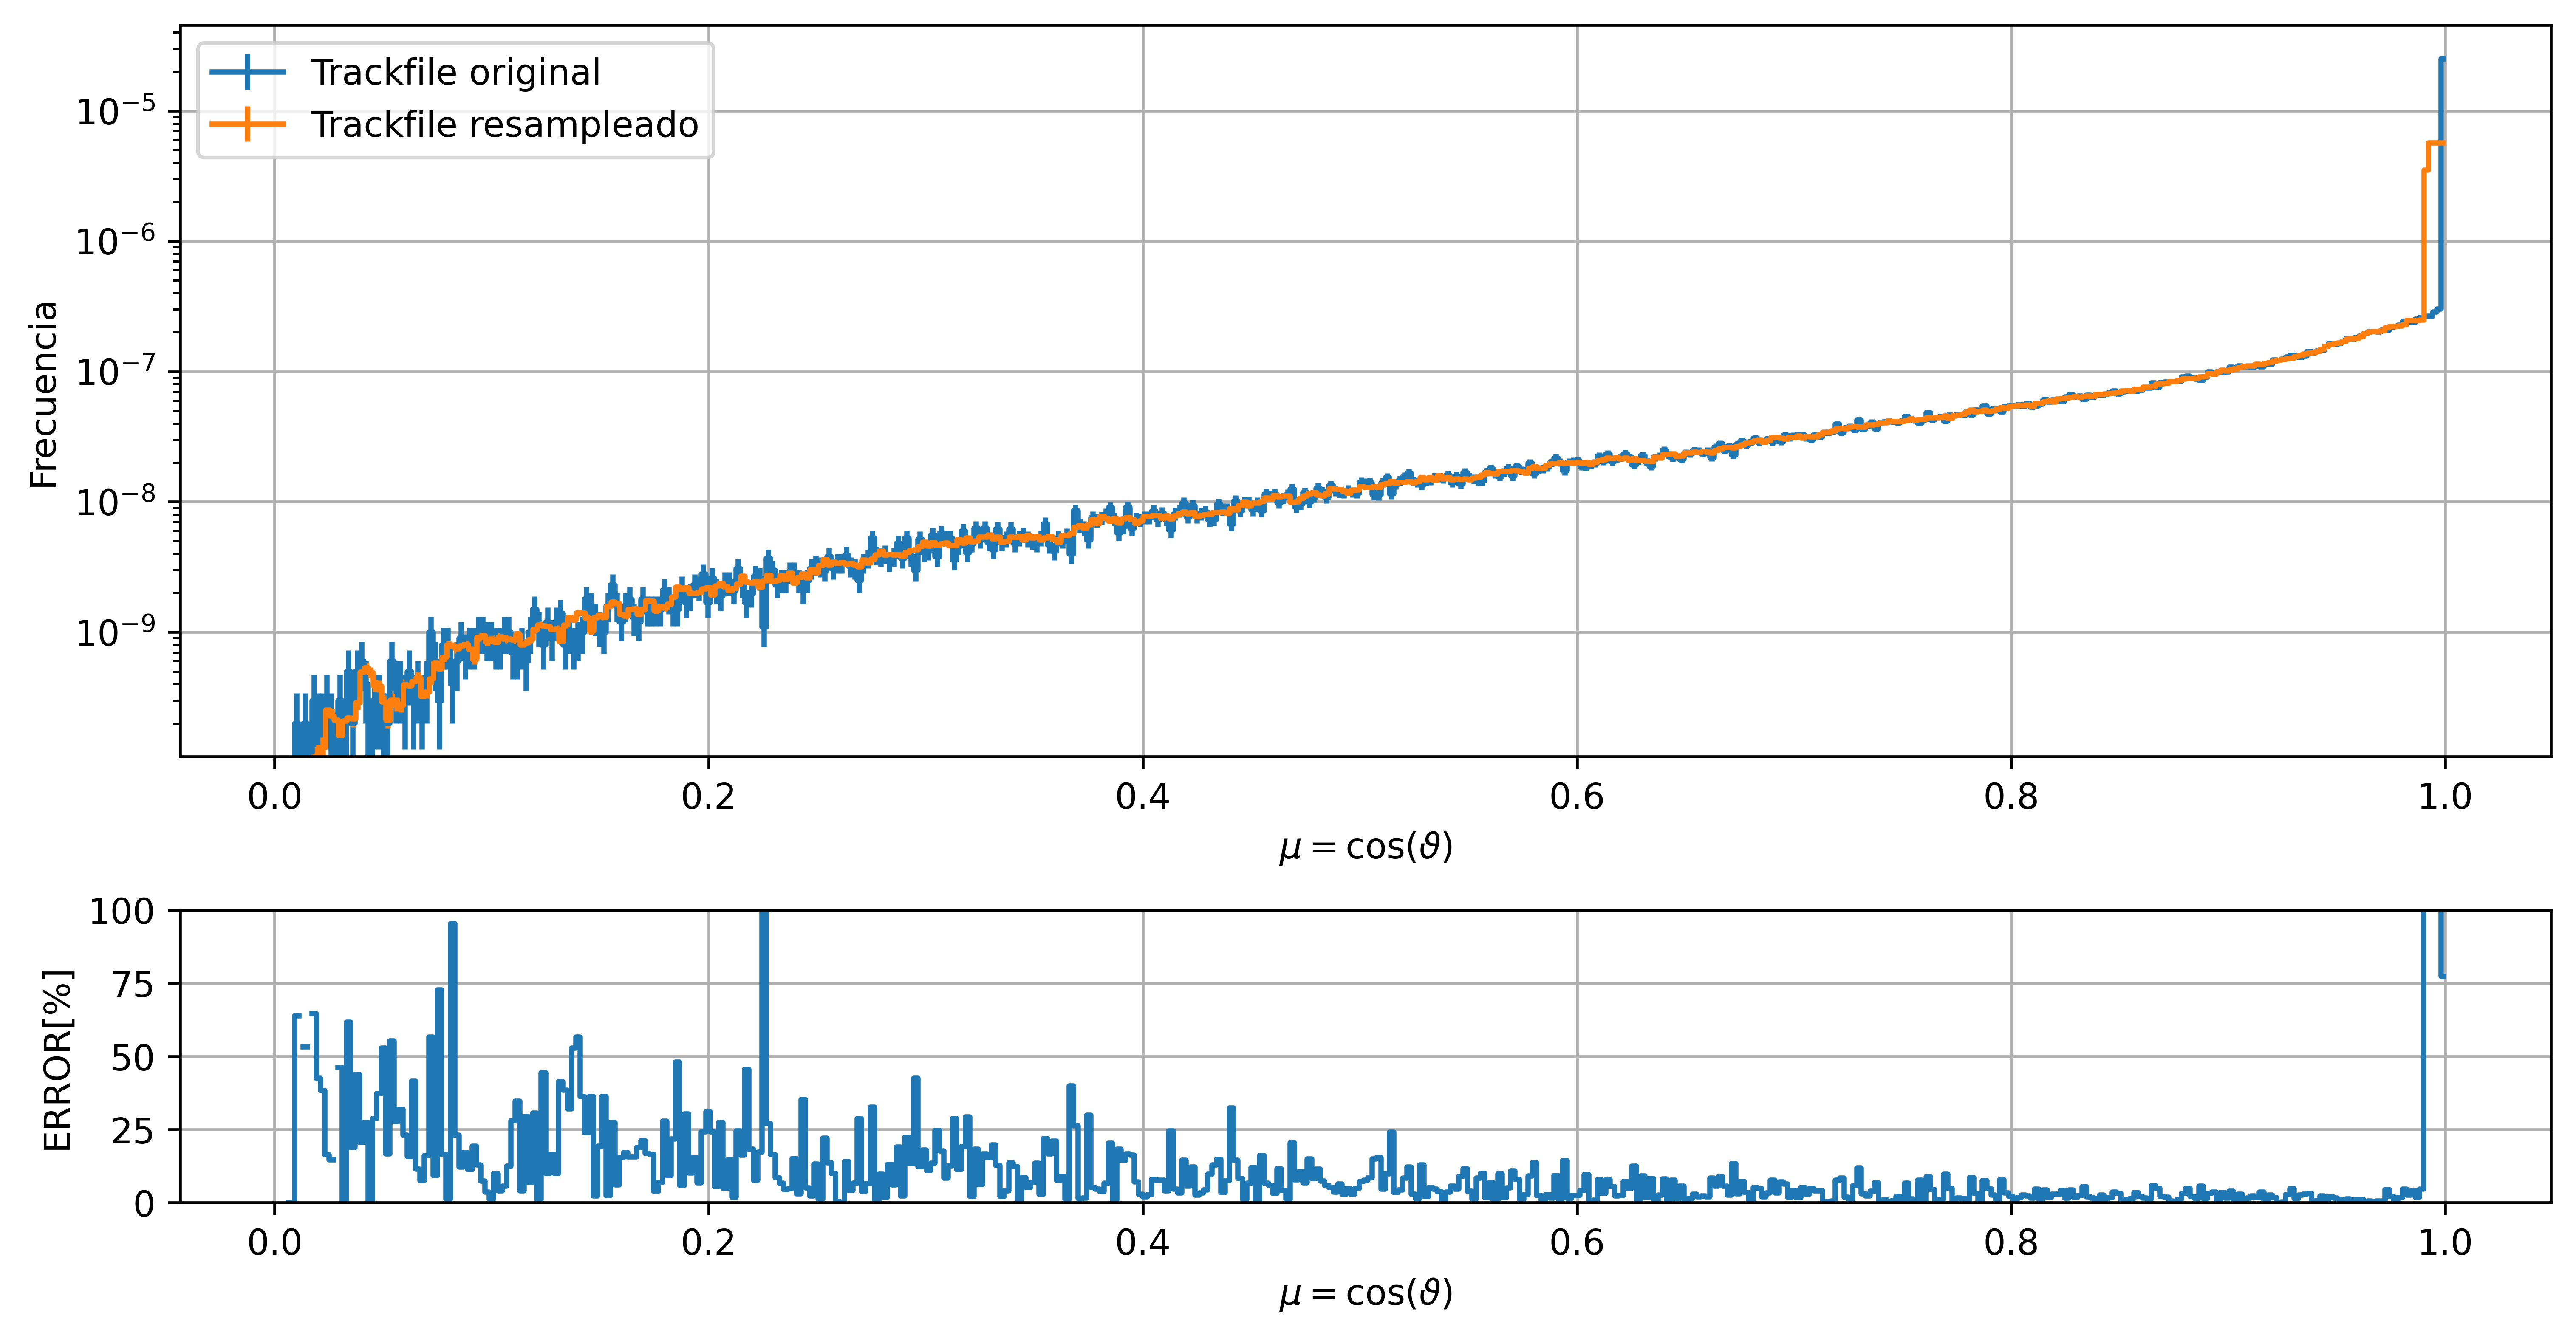
\includegraphics[width=\textwidth]{figs/fig2_5.png}
    \caption{Comparacion de la distribucion de mu entre el trackfile original y el trackfile remuestreado. Se observa el efecto de la discretizacion uniforme en la distribucion de mu.}
    \label{fig:trackfile1_config1_mu}
\end{figure}

Además, en las distribuciones espaciales, tanto $x$ como $y$, se elimina el ruido estadístico original de forma local pero sin suavizado general, reflejando el bineado uniforme. Esto se observa en la figura \ref{fig:trackfile1_config1_x}, donde se comparan las distribuciones de $x$ entre el trackfile original y el remuestreado. 

\begin{figure}[h]
    \centering
    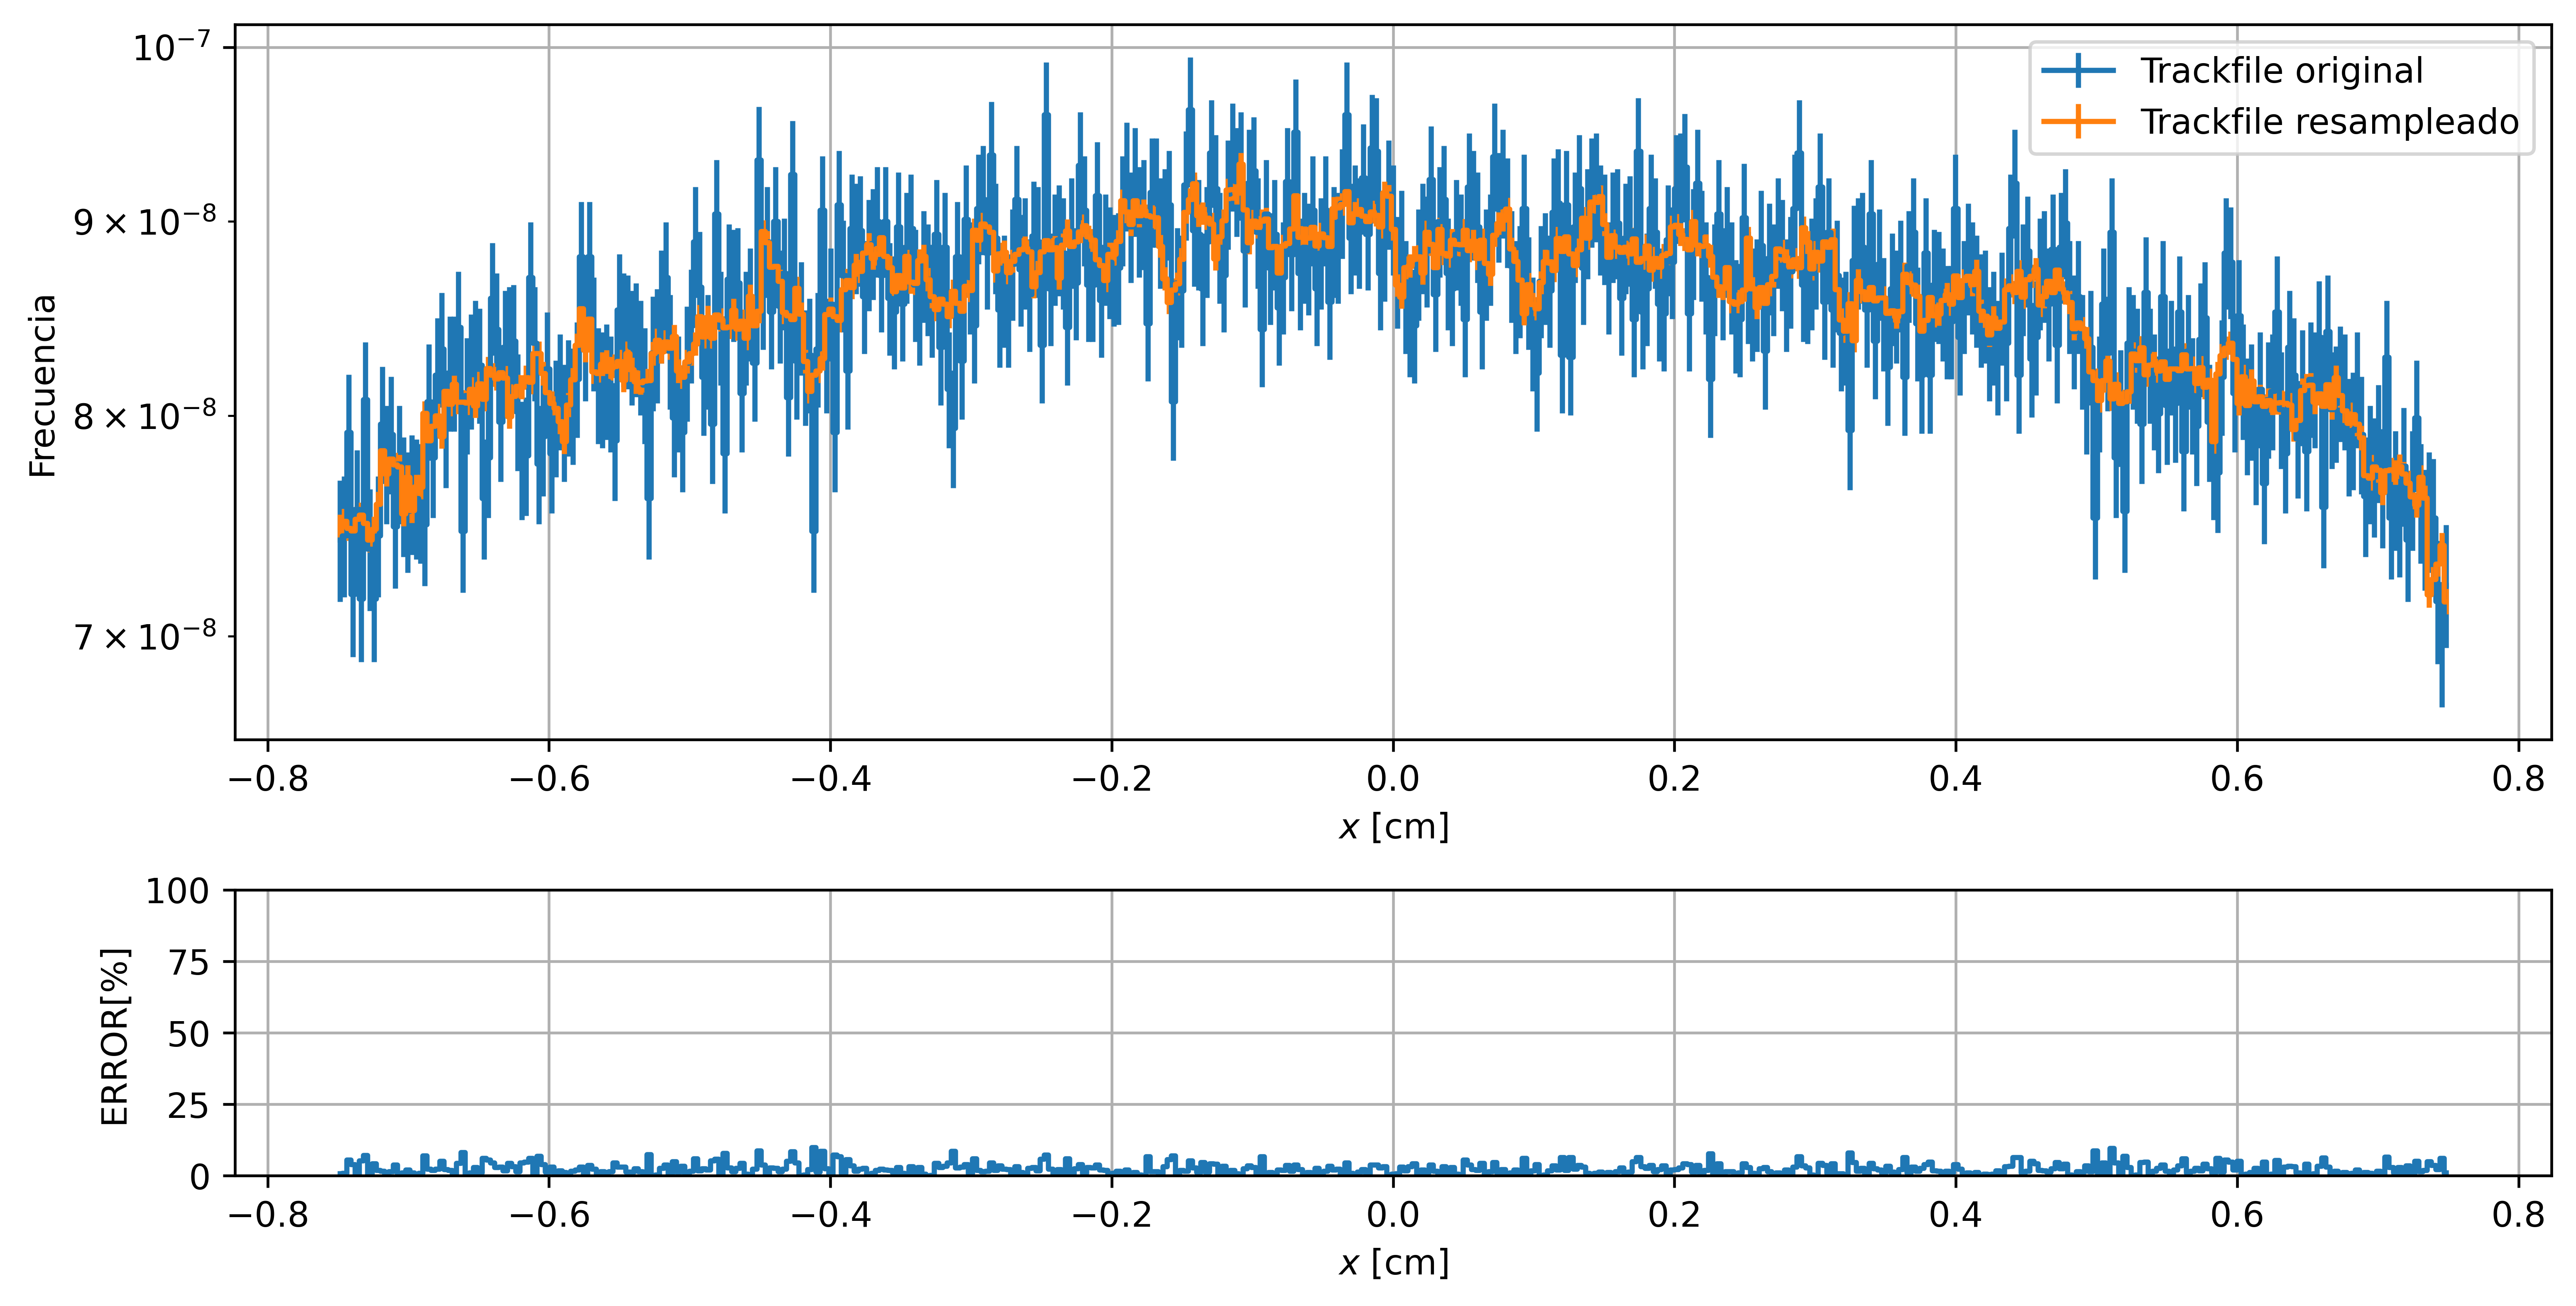
\includegraphics[width=\textwidth]{figs/fig2_6.png}
    \caption{Comparacion de la distribucion de x entre el trackfile original y el trackfile remuestreado. Se observa el efecto de la discretizacion uniforme en la distribucion de x debido a que se reduce el ruido a nivel local pero se observa el bineado uniforme.}
    \label{fig:trackfile1_config1_x}
\end{figure}

Las métricas KL resultantes indican errores importantes en variables con alta concentración, especialmente en $\mu$ y letargia, tanto en 1D como en 2D:

\begin{table}[h]
    \centering
    \caption{Divergencia KL parcial y total para la configuración \texttt{Equal / Equal}.}
    \label{tab:KL_parciales_equal_columns}
    \begin{tabular}{llr@{\hspace{2cm}}llr}
    \toprule
    \multicolumn{2}{c}{\textbf{KL 1D}} & \multicolumn{2}{c}{\textbf{KL 2D}} \\
    \cmidrule(lr){1-2} \cmidrule(lr){3-4}
    \textbf{Parámetro} & \textbf{Valor} & \textbf{Parámetros} & \textbf{Valor} \\
    \midrule
    $\ln(E_0/E)$ & 1.2229 & $\ln(E_0/E), x$    & 1.6981 \\
    $x$          & 1.0918e-03 & $\ln(E_0/E), y$    & 1.7038 \\
    $y$          & 1.0679e-03 & $\ln(E_0/E), \mu$  & 3.8917 \\
    $\mu$        & 1.1957 & $\ln(E_0/E), \phi$ & 3.6191 \\
    $\phi$       & 1.4702 & $x, y$             & 1.1812 \\
       &              & $x, \mu$           & 2.0564 \\
       &              & $x, \phi$          & 2.4558 \\
       &              & $y, \mu$           & 2.0566 \\
       &              & $y, \phi$          & 2.4674 \\
       &              & $\mu, \phi$        & 3.9723 \\
    \midrule
    \textbf{Suma KL 1D} & \textbf{3.8909} & \textbf{Suma KL 2D} & \textbf{25.102} \\
    \bottomrule
    \end{tabular}
\end{table}

% \begin{table}[H]
%     \centering
%     \caption{Divergencia KL parcial para configuración \texttt{Equal / Equal}.}
%     \label{tab:KL_parciales_equal_columns}
%     \begin{tabular}{llr@{\hspace{2cm}}llr}
%     \toprule
%     \multicolumn{2}{c}{\textbf{KL 1D}} & \multicolumn{2}{c}{\textbf{KL 2D}} \\
%     \cmidrule(lr){1-2} \cmidrule(lr){3-4}
%   \textbf{Parámetro} & \textbf{Valor} & \textbf{Parámetros} & \textbf{Valor} \\
%     \midrule
%     $\ln(E_0/E)$ & 1.2229 & $\ln(E_0/E), x$    & 1.6981 \\
%     $x$          & 1.0918e-03 & $\ln(E_0/E), y$    & 1.7038 \\
%     $y$          & 1.0679e-03 & $\ln(E_0/E), \mu$  & 3.8917 \\
%     $\mu$        & 1.1957 & $\ln(E_0/E), \phi$ & 3.6191 \\
%     $\phi$       & 1.4702 & $x, y$             & 1.1812 \\
%        &              & $x, \mu$           & 2.0564 \\
%        &              & $x, \phi$          & 2.4558 \\
%        &              & $y, \mu$           & 2.0566 \\
%        &              & $y, \phi$          & 2.4674 \\
%        &              & $\mu, \phi$        & 3.9723 \\
%     \bottomrule
%     \end{tabular}
%     \end{table}
    

% \begin{center}
% \begin{tabular}{lcc}
% \toprule
% \textbf{Configuración} & $\sum$KL 1D & $\sum$KL 2D \\
% \midrule
% Equal / Equal & 3.89 & 25.10 \\
% \bottomrule
% \end{tabular}
% \end{center}

\paragraph{Configuración 2: binning adaptativo (adaptive/adaptive).}  
Al aplicar binning adaptativo tanto en los macrogrupos como microgrupos, se optimiza la ubicación de los bordes para reflejar mejor la densidad local. En letargia se observa una mejora sustancial en la representación de los valores tipo delta, aunque persisten irregularidades en las zonas de letargia alta. Las variables espaciales muestran una mayor suavidad local sin perder detalle global.

Las métricas KL mejoran drásticamente respecto del caso uniforme:

\begin{center}
\begin{tabular}{lcc}
\toprule
\textbf{Configuración} & $\sum$KL 1D [nats] & $\sum$KL 2D [nats] \\
\midrule
Adaptive / Adaptive & 0.533 & 10.15 \\
\bottomrule
\end{tabular}
\end{center}

\paragraph{Configuración 3: macrobinning adaptativo, microbinning uniforme.}  
Esta variante mejora parcialmente la resolución estructural de la distribución, especialmente en 2D, pero mantiene el error en 1D cuando hay discontinuidades abruptas. Esto se refleja en un KL total intermedio:

\begin{center}
\begin{tabular}{lcc}
\toprule
\textbf{Configuración} & $\sum$KL 1D [nats] & $\sum$KL 2D [nats] \\
\midrule
Adaptive / Equal & 1.087 & 12.56 \\
\bottomrule
\end{tabular}
\end{center}

\paragraph{Configuración 4: macrobinning uniforme, microbinning adaptativo.}  
Esta última configuración aún no ha sido evaluada en detalle, pero se espera que muestre un comportamiento intermedio entre los casos previos. Se incluirá su análisis en una versión posterior.



\section{Resultados con Trackfile 1}
\label{sec:resultados-track1}

En esta sección se presentan los resultados obtenidos al aplicar el método sobre el primer archivo de tracks. El análisis se realizó utilizando múltiples configuraciones, variando el orden de las variables, la cantidad de macrogrupos y microgrupos.

Se muestran:

\begin{itemize}
    \item Distribuciones de energía, posición y dirección reconstruidas y su comparación con las originales.
    \item Curvas de error relativo por variable.
    \item Mapas de error relativo 2D para las correlaciones seleccionadas.
    \item Tabla con valores de divergencia KL para distintas configuraciones.
\end{itemize}

Estos resultados permiten discutir la sensibilidad del método a cada uno de los parámetros de entrada y establecer lineamientos para su elección óptima.

\subsection{Comparación entre esquema adaptativo y de ancho constante}
\label{subsec:adaptativo-vs-constante}

Como parte del análisis sobre el primer trackfile, se estudió el impacto del esquema de discretización utilizado en los macro y microgrupos. Se comparó explícitamente el rendimiento del esquema adaptativo frente a un esquema de histogramas con ancho constante.

El esquema adaptativo asigna mayor resolución a regiones del espacio de fases con alta estadística, y menor resolución donde los datos son escasos. Esto permite representar con mayor fidelidad las distribuciones sin amplificar el ruido estadístico.

Los resultados muestran una mejora significativa en la reconstrucción cuando se utiliza el esquema adaptativo. Esto se evidencia tanto en los gráficos de error relativo como en los valores de la divergencia KL, donde se observa una reducción consistente al aplicar el bineado adaptativo.

% \begin{figure}[H]
%     \centering
%     \includegraphics[width=0.75\textwidth]{figuras/ejemplo_adaptativo_vs_constante.png}
%     \caption{Comparación entre esquema adaptativo (izquierda) y esquema de ancho constante (derecha) en una variable espacial. Se observa mejor resolución en regiones con alta densidad de partículas.}
%     \label{fig:adaptativo-vs-constante}
% \end{figure}

Esta comparación resalta la importancia de emplear técnicas de bineado adaptativo como herramienta para preservar la calidad del muestreo, especialmente en regiones con estructuras finas y alta variabilidad estadística.

\section{Resultados con Trackfile 2}
\label{sec:resultados-track2}

Se repitió el procedimiento metodológico sobre un segundo archivo de tracks con características geométricas y espectrales diferentes al primero, lo cual permite poner a prueba la generalidad del método propuesto.

Al igual que en el caso anterior, se analizaron distintas configuraciones de discretización jerárquica y orden de variables, prestando especial atención a:

\begin{itemize}
    \item La estabilidad del método ante distribuciones menos suaves o más concentradas espacialmente.
    \item La sensibilidad de las correlaciones bidimensionales al cambio en el esquema de macrogrupos.
    \item El comportamiento de la divergencia KL como función de la resolución utilizada.
\end{itemize}

Los gráficos comparativos muestran una buena reconstrucción general de las distribuciones 1D, aunque se observaron mayores errores relativos en regiones de baja estadística. En cuanto a las correlaciones, se destaca nuevamente la importancia de evitar configuraciones con fragmentación excesiva en las últimas variables del árbol.

Se presenta a continuación una selección representativa de los resultados gráficos y numéricos obtenidos, incluyendo:

\begin{itemize}
    \item Plots de distribuciones originales vs. reconstruidas.
    \item Mapas de error relativo 2D para variables espaciales y angulares.
    \item Tabla comparativa de divergencias KL.
\end{itemize}

% \begin{figure}[H]
%     \centering
%     \includegraphics[width=0.8\textwidth]{figuras/trackfile2_errores.png}
%     \caption{Error relativo en la distribución de la variable $\mu$ para distintas configuraciones en Trackfile 2.}
%     \label{fig:trackfile2_mu}
% \end{figure}

\begin{table}[H]
    \centering
    \caption{Divergencia KL para distintas configuraciones en Trackfile 2.}
    \begin{tabular}{lccc}
        \toprule
        \textbf{Configuración} & \textbf{Macrogrupos} & \textbf{Microgrupos} & \textbf{KL Divergence} \\
        \midrule
        Orden A & [8,8,8,8] & [80,80,80,80] & 0.021 \\
        Orden B & [6,7,8,9] & [60,70,80,90] & 0.016 \\
        Orden C & [9,8,7,6] & [100,80,60,40] & 0.019 \\
        \bottomrule
    \end{tabular}
    \label{tab:trackfile2_kl}
\end{table}


\section{Resultados con Trackfile 3}
\label{sec:resultados-track3}

Finalmente, se aplicó el método sobre un tercer archivo de tracks con características mixtas, presentando una distribución energética más extendida y un patrón angular complejo, lo cual representa un desafío adicional para el muestreo jerárquico.

Se realizaron pruebas similares a las anteriores, enfocándose en:

\begin{itemize}
    \item Evaluar la robustez del método frente a distribuciones con múltiples picos o simetrías rotas.
    \item Observar el efecto del esquema de macrogrupos decreciente en variables angulares.
    \item Validar si se mantiene la tendencia en la divergencia KL al aplicar bineado adaptativo.
\end{itemize}

Los resultados obtenidos son consistentes con los de los otros casos, aunque se observaron diferencias notables en la reconstrucción de las variables angulares cuando éstas se encontraban en posiciones tempranas dentro del árbol, lo cual sugiere una posible pérdida de fidelidad debido a fragmentación excesiva.

% \begin{figure}[H]
%     \centering
%     \includegraphics[width=0.75\textwidth]{figuras/trackfile3_phi.png}
%     \caption{Distribución reconstruida de la variable $\phi$ en Trackfile 3 con esquema adaptativo.}
%     \label{fig:trackfile3_phi}
% \end{figure}

\begin{table}[H]
    \centering
    \caption{Divergencia KL en Trackfile 3 para diferentes combinaciones.}
    \begin{tabular}{lccc}
        \toprule
        \textbf{Configuración} & \textbf{Macrogrupos} & \textbf{Microgrupos} & \textbf{KL Divergence} \\
        \midrule
        Esquema uniforme & [6,6,6,6] & [60,60,60,60] & 0.024 \\
        Esquema creciente & [6,7,8,9] & [60,70,80,90] & 0.017 \\
        Esquema adaptativo & Variable & Adaptativo & 0.012 \\
        \bottomrule
    \end{tabular}
    \label{tab:trackfile3_kl}
\end{table}

Estos resultados reafirman la utilidad del esquema adaptativo en escenarios complejos, donde las estructuras locales en el espacio de fases requieren una resolución flexible para ser correctamente representadas.


